%
% This is Chapter 3 file (chap3.tex)
%
\chapter{Reproducibility Study using Unified IR Evaluation System}

Developing effective information retrieval models has been a 
long standing challenge in Information Retrieval (IR), and significant 
progresses have been made over the years. With the increasing 
number of developed retrieval functions and the release of 
new data collections, it becomes more difficult, if not impossible, 
to compare a new retrieval function with all existing retrieval 
functions over all available data collections.  
The context -- the evaluation system is crucial to solving this problem.
To tackle this problem, we construct the unified IR evaluation systems 
that aim to improve the reproducibility of IR research
and facilitate the evaluation and comparison of retrieval functions. 
With the developed platform, more than 20 state of the art 
retrieval functions have been implemented and systematically 
evaluated over 16 standard TREC collections (including the newly 
released ClueWeb datasets). Our reproducibility study leads to 
several interesting observations. First, the performance difference
between the reproduced results and those reported in the original 
papers is small for most retrieval functions.  Second, the optimal 
performance of a few representative retrieval functions is still 
comparable over the new TREC ClueWeb collections. 
Finally, the developed platform (i.e., {\em RISE}) is made publicly 
available so that any IR researchers would be able to utilize 
it to evaluate other retrieval functions. 


\section{VIRLab}

Existing IR toolkits do not offer an easy solution for users 
to implement, evaluate and analyze new retrieval models, 
which often pose unnecessary extra burdens to the users. 
For example, users need to learn how to access various term 
or document statistic information from the index, and read 
through source codes or API documentations to figure out how 
to implement a new retrieval function. After implementing the 
function, the users often need to write their own scripts to 
evaluate and analyze the search results over multiple collections. 
This kind of process adds unnecessary burden to the users and 
could discourage them from experimenting with more functions 
over more collections. Naturally, it is also very challenging 
to use such toolkits for a course assignment.

In this section we describe our efforts on developing a web-based
tool for IR students or researchers to study retrieval functions 
in a more interactive and cost-effective way. We will
demonstrate that the developed system, i.e,. Virtual IR Lab
(VIRLab), can offer the following new functionalities:

\begin{itemize}
\item \textit{Easy implementation of retrieval functions}: 
Users only need to write a few lines of code through a Web form
to combine statistics retrieved from the indexes without 
worrying about how to access the indexes. The code will be 
automatically checked for syntax errors and translated to an 
executable, which will be used for ranking documents, 
by a dynamic code generator.
\item \textit{Flexible configuration of search engines}: 
Users can configure a search engine by selecting a retrieval 
function and a test collection. Multiple search engines can be
easily created at the same time. The users can either submit 
their own queries or select queries from a set of topics 
associated with the corresponding document collection. 
Moreover, the users can also compare the search results 
of two search engines side by side to figure out their 
ranking differences.
\item \textit{Tight connections among implementation, evaluation
and result analysis}: 
After creating a retrieval function, the users can evaluate its 
effectiveness over a few provided test collections by simply 
clicking a button. If a retrieval function contains multiple 
parameter values, the users may select to evaluate all of them. 
If a search engine is configured using an existing test collection 
with relevance judgments, the official queries and judgments 
will be displayed so that the users can easily analyze the search 
results to figure out when the search engine fails and why.
\item \textit{Performance comparison through leader-boards}: 
A leader board is created for each collection so that the most
effective 10 retrieval functions are displayed. Users
can see how their retrieval functions are compared with
others, and they can also leverage the comparison functionality 
described earlier to figure out how to revise
their retrieval functions to improve the performance.
\end{itemize}

\section{RISE - A Reproducibility Platform for Retrieval Models} 
\label{sec:system}

To reproduce the results of retrieval models, we implement 
a web-based Reproducible Information retrieval System Evaluation ({\em RISE}) 
platform.  The platform is designed to provide a well-controlled 
environment for the users to implement and evaluate retrieval functions.  
Figure \ref{fig:system} shows the architecture of RISE. 
{\em RISE} is basically a web service built on top of a modified 
version of the Indri\footnote{http://sourceforge.net/projects/lemur/} toolkit. 
{\em RISE} hosts data collections on the server side, processes documents, 
and builds the indexes.
Users need to upload their own implementations 
of retrieval functions based on the provided templates.  
After the code is uploaded,  {\em RISE} automatically compiles it and 
evaluates it over the selected data collections. 
The evaluation results of the retrieval function will 
then be added to the score boards and thus be available for comparison.   

\begin{figure}[t]
\centering
    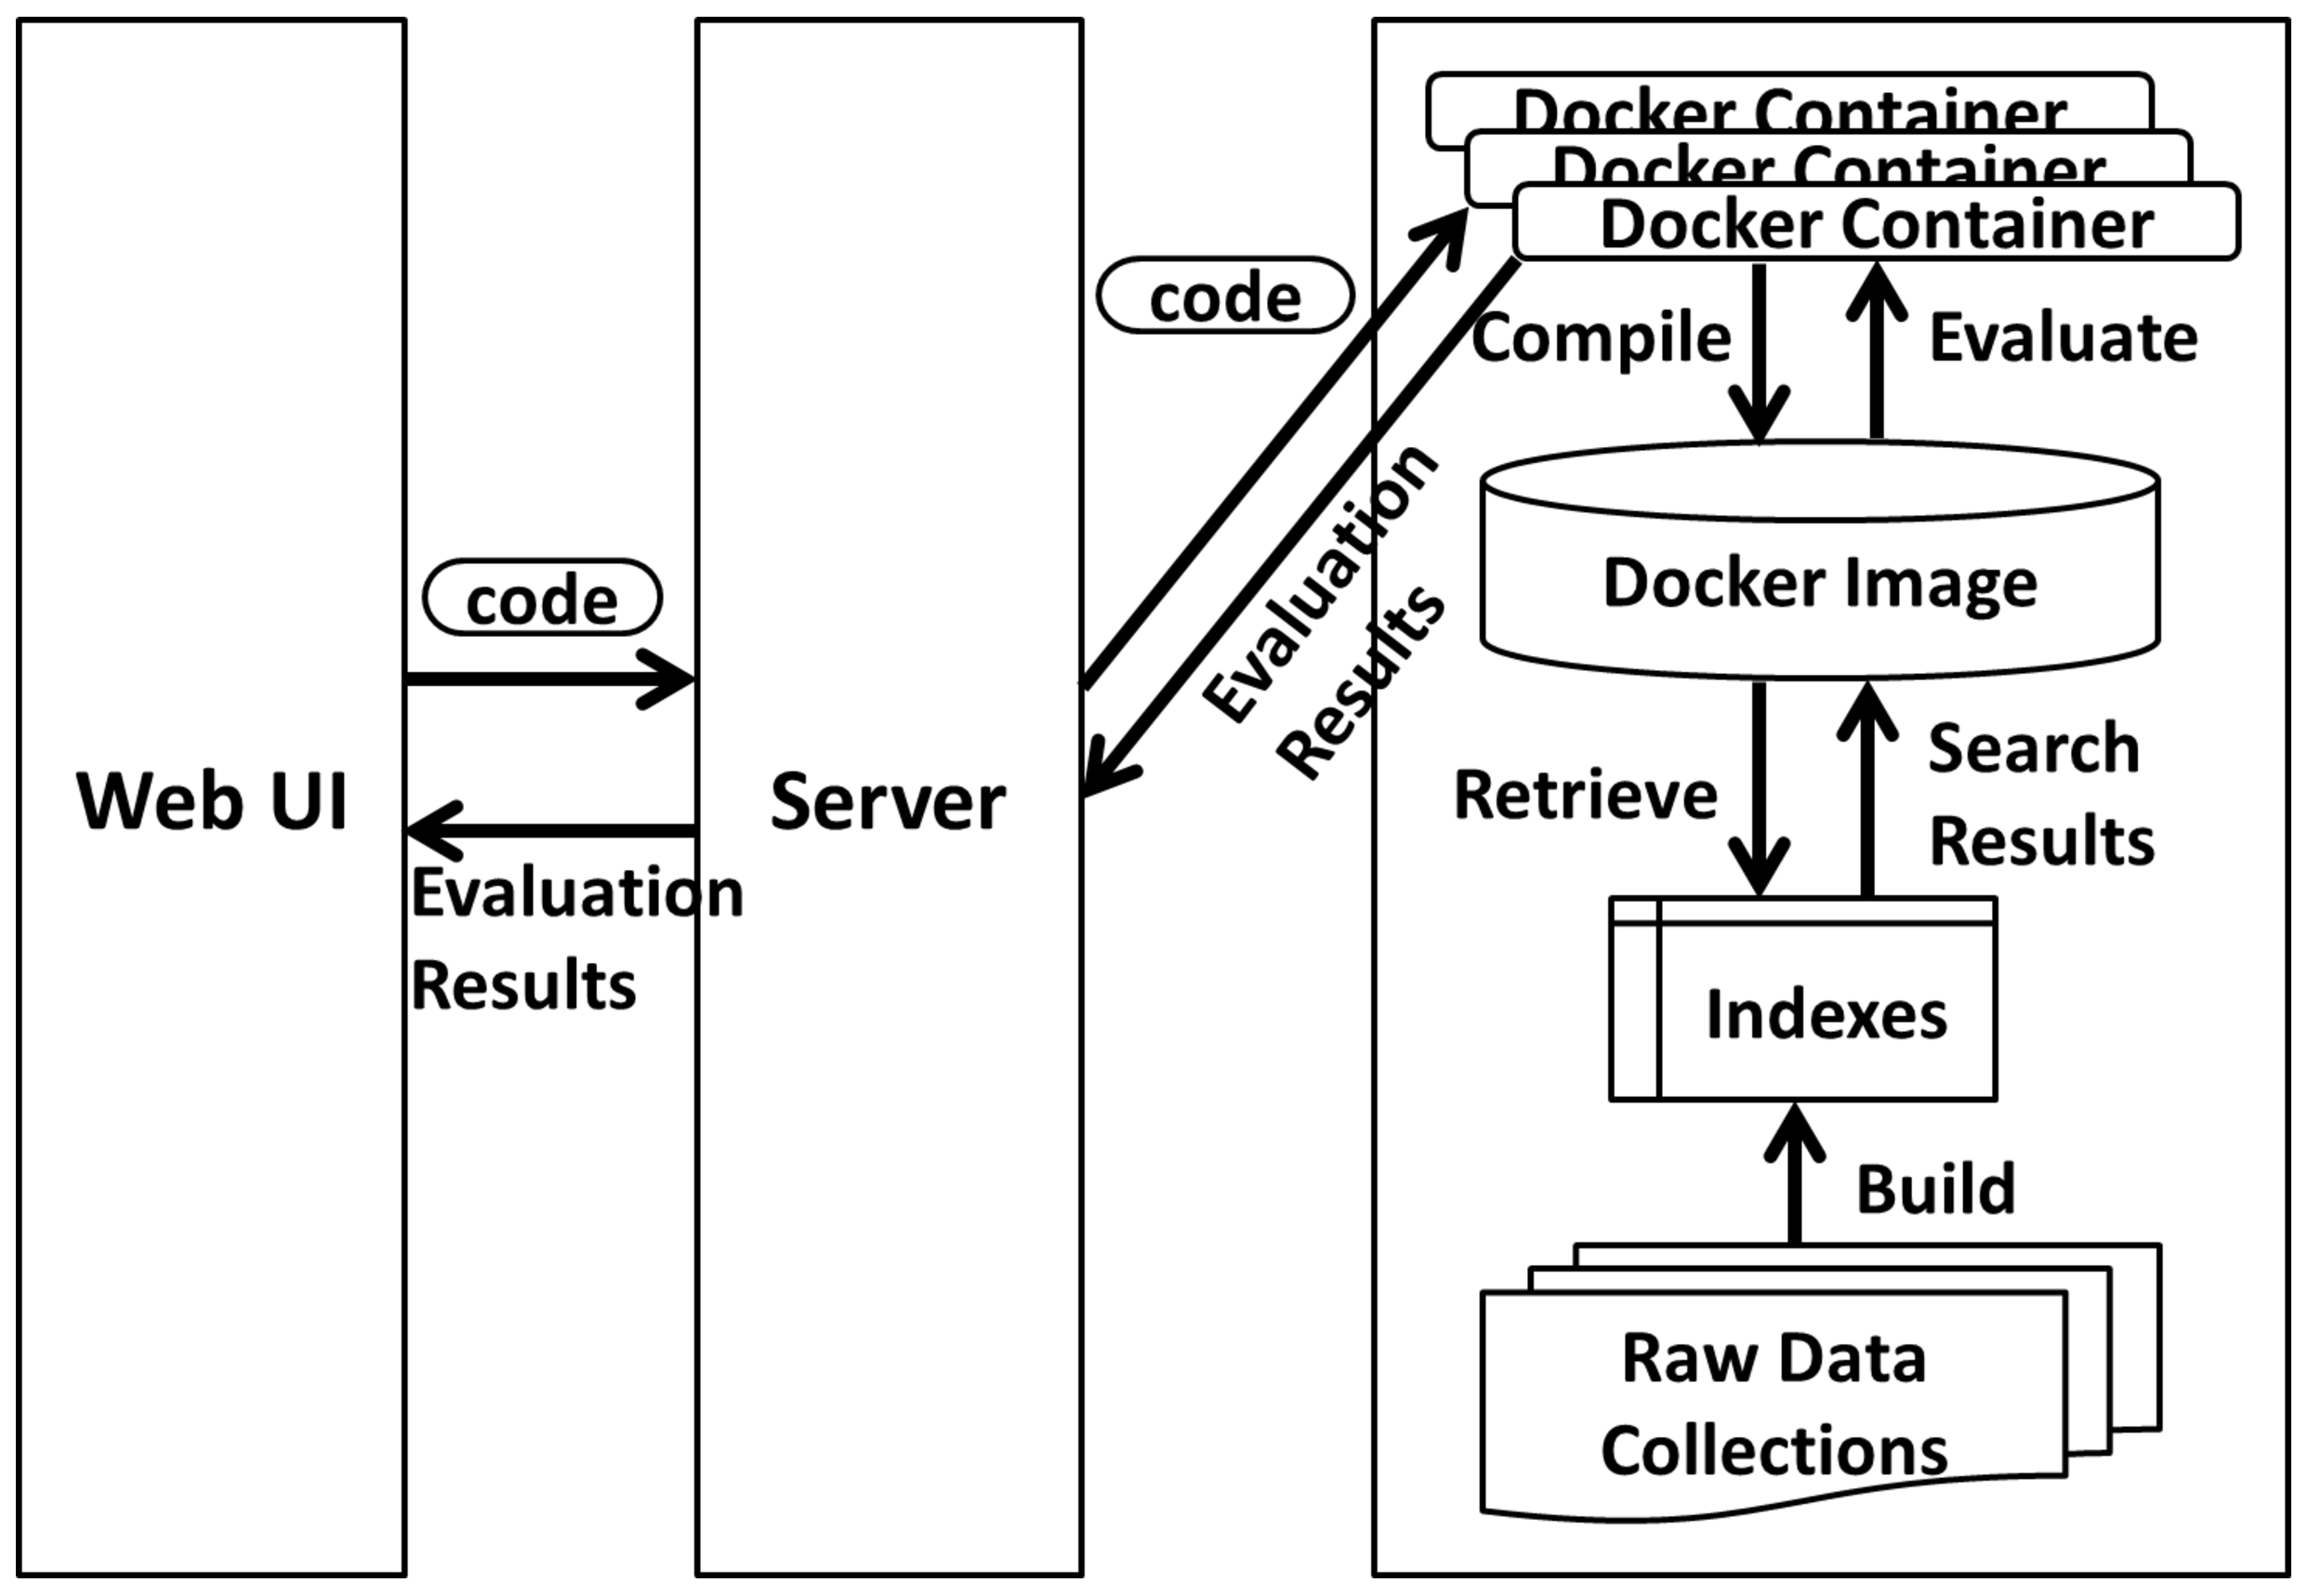
\includegraphics[width=1.0\textwidth]{figures/RISE.eps}
    \caption{System Architecture\label{fig:system}}
\end{figure}

Any registered users can contribute the implementation of 
a retrieval model to the system. Users are 
expected to be familiar with C++ but not necessarily 
familiar with Indri, as we provide detailed instructions with sample codes on how to 
access the statistics from the indexes and how to implement ranking models with 
the provided statistics.  Moreover, {\em RISE} is an open system which 
allows any user to view any other users' implementations of the models.  
This functionality makes it possible for a user to easily try 
different variants of existing retrieval functions. 
The modified version of the Indri toolkit provides various 
statistics that are not available in the original version. 
These new statistics include query term frequency, average document term 
frequency, etc. 

After the code is submitted to the server and successfully 
compiled, a Docker container 
is temporarily initiated on top of the static Docker image. 
(Docker container is like a sandbox which provides an isolated 
environment acting like an operating system. For more information 
please refer to https://www.docker.com/) 
The Docker image includes the indexes built from data collections 
and the modified Indri toolkit that will be used as the facility to 
run the model and generate the ranking list. 
A Docker image can be utilized by several Docker containers at the 
same time while keep the same underlying view of index and thus is 
the ideal choice for the system. 
Several Docker containers can be initiated in 
parallel so that multiple models can be compiled, run and evaluated 
at the same time. Moreover, by carefully setting the Docker container 
we can control the CPU and memory usage as well as security 
related settings (e.g. network, 3rd party libraries) so that the 
system is more robust against malicious/careless usage. 
The running Docker container compiles the codes, generate the ranking 
list, then evaluate the results. After that, the performance is 
rendered to the users and users can opt to choose other models to compare with. 

%To summarize, {\em RISE} has the following properties:  
%\begin{itemize}
%\item Adopt the design of web service which requires minimum effort 
%for the user to implement IR ranking models
%\item Use modified Indri as the underlying toolkit which provides 
%more statistics that user can leverage
%\item Is in terms of the visibility of the implementations: code 
%submitted by one user is available to be reviewed by all other users
%\item Use Docker to control the evaluation environment which is more 
%secure, faster and reliable
%\end{itemize}


There are several major benefits of the developed {\em RISE} platform.  
(1) The data collections are kept on the server side to preserve
the data privacy.  (2) The platform uses Docker to control the 
evaluation environment, which is more secure, faster and more 
reliable.  
(3) The platform provides 
a repository of the implementation of various retrieval functions. 
Registered users can upload their own codes, and these codes can be 
reused by other users.  Such a repository could eliminate redundant 
efforts of implementing baseline methods among IR researchers. 
(4) The platform maintains the scores for each implemented retrieval 
function over all available data sets.  The score boards could become
a valuable reference when a new retrieval function needs to be evaluated
and compared with the state of the art methods. 


%Apparently, there are more nice-to-have features for RISE. 
%For example, split the training and the testing collections 
%which makes the parameter tuning more easily or otherwise user needs 
%to brute force the parameters. We leave such job as the future work. 

\newcommand{\specialcell}[2][c]{%
  \begin{tabular}[#1]{@{}c@{}}#2\end{tabular}}
    \begin{table*}[t]
    \caption{Retrieval functions that are reproduced in our study (Part 1)\label{tab:allmodels}}
    \centering
    \begin{tabular}{ |l|c| }
     \hline
    \multicolumn{2}{|c|}{Okapi BM25 and its variants} \\ \hline
    BM25 & $
    \sum_{t \in q} {\frac{(k_3+1)\cdot c_{t}^{q}}{k_3+c_{t}^{q}}}\cdot \frac{(k_1+1) \cdot c_{t}^{d}}{c_{t}^{d} + k_1 \cdot (1-b+b\cdot \frac{l_{d}}{L})} \cdot ln \Big(\frac{N-N_{t}+0.5}{N_{t}+0.5}\Big) 
    $ \\ \hline

    F2EXP & $
    \sum_{t \in q}{\frac{c_{t}^{d}}{c_{t}^{d}+s+s\cdot \frac{l_{d}}{L}}}\cdot \Big(\frac{N+1}{N_t}\Big)^k
    $ \\ \hline

    F2LOG & $
    \sum_{t \in q}{\frac{c_{t}^{d}}{c_{t}^{d}+s+s\cdot \frac{l_{d}}{L}}}\cdot ln\Big(\frac{N+1}{N_t}\Big)
    $ \\ \hline

    \multirow{2}{*}{BM3} & $
    \sum_{t \in q} {\frac{(k_3+1)\cdot c_{t}^{q}}{k_3+c_{t}^{q}}}\cdot \frac{(k_1+1) \cdot tfn}{k_1+tfn} \cdot ln \Big(\frac{N-N_{t}+0.5}{N_{t}+0.5}\Big)
    $ \\ 
    & $
    tfn = \frac{c_{t}^{d}+\mu \cdot \frac{F_t}{|C|}}{l_{d}+\mu}\cdot \mu
    $ \\ \hline

    BM25+ & $
    \sum_{t \in q} {\frac{(k_3+1)\cdot c_{t}^{q}}{k_3+c_{t}^{q}}} \cdot \Big[\frac{(k_1+1) \cdot c_{t}^{d}}{c_{t}^{d} + k_1 \cdot (1-b+b \cdot \frac{l_{d}}{L})}+\delta\Big] \cdot ln (\frac{N+1}{N_{t}})
    $ \\ \hline
         \hline

    \multicolumn{2}{|c|}{Pivoted and its variants} \\ \hline 
    PIV & $
    \sum_{t \in q}{\frac{1+ln(1+ln(c_{t}^{d}))}{(1-s)+s\cdot \frac{l_{d}}{L}} \cdot ln \Big(\frac{N+1}{N_{t}}\Big)}
    $ \\ \hline

    F1EXP & $
    \sum_{t \in q}{(1+ln(1+ln(c_{t}^{d})))\cdot \frac{L+s}{L+s\cdot l_{d}} \cdot \Big(\frac{N+1}{N_t}\Big)^k}
    $ \\ \hline

    F1LOG & $
    \sum_{t \in q}{(1+ln(1+ln(c_{t}^{d})))\cdot \frac{L+s}{L+s\cdot l_{d}} \cdot ln\Big(\frac{N+1}{N_t}\Big)}
    $ \\ \hline

    PIV+ & $
    \sum_{t \in q}{\Big[\frac{1+ln(1+ln(c_{t}^{d}))}{(1-s)+s\cdot \frac{l_{d}}{L}} + \delta \Big] \cdot ln \Big(\frac{N+1}{N_{t}}\Big)}
    $ \\ \hline

    \multirow{2}{*}{NTFIDF} & $
    \sum_{t \in q} \Bigg[\Big[\omega \cdot f\Big(\frac{c_{t}^{d}}{l_{d}/c_d}\Big) + (1-\omega)\cdot f\Big(c_{t}^{d}\cdot log_2\Big(1+\frac{L}{l_{d}}\Big)\Big)\Big] \cdot \Big[ln\Big(\frac{N+1}{N_t}\Big) \cdot f\Big(\frac{F_t}{N_t}\Big)\Big]\Bigg]$ \\ 
    & $\omega=\frac{2}{1+log_2(1+|q|)}$, $f(x)=\frac{x}{1+x}$ \\ \hline
         \hline
    \end{tabular} 
    \end{table*}

    \begin{table*}[t]
    \caption{Retrieval functions that are reproduced in our study (Part 2)\label{tab:allmodels2}}
    \centering
    \begin{tabular}{ |l|c| }
     \hline
    \multicolumn{2}{|c|}{Language modeling approaches} \\ \hline 
    DIR & $
    \sum_{t \in q}{ln\Big(\frac{c_{t}^{d}+\mu \cdot \frac{F_t}{|C|}}{l_{d}+\mu}\Big)}
    $ \\ \hline

    TSL & $
    \sum_{t \in q}{((1-\lambda)\cdot \frac{c_{t}^{d}+\mu \cdot \frac{F_t}{|C|}}{l_{d}+\mu}+\lambda \cdot \frac{F_t}{|C|})}
    $ \\ \hline

    BLM & $
    \sum_{t \in q}{\frac{c_{t}^{d}+\mu \cdot \frac{F_t}{|C|}}{l_{d}+\frac{|C|}{F_t}+\mu-2} }
    $ \\ \hline

    F3EXP & $
    \sum_{t \in q}{(1+ln(1+ln(c_{t}^{d})))\cdot \Big(\frac{N+1}{N_t}\Big)^k} - \frac{(l_{d}-|q|)\cdot |q|\cdot s}{L}
    $ \\ \hline

    F3LOG & $
    \sum_{t \in q}{(1+ln(1+ln(c_{t}^{d})))\cdot ln\Big(\frac{N+1}{N_t}\Big)} - \frac{(l_{d}-|q|)\cdot |q|\cdot s}{L}
    $ \\ \hline

    DIR+ & $
    \sum_{t \in q} \Big[ln\Big(1+\frac{c_{t}^{d}}{\mu \cdot \frac{F_t}{|C|}}\Big)+ln\Big(1+\frac{\delta}{\mu \cdot \frac{F_t}{|C|}}\Big)\Big] +|q|\cdot ln\frac{\mu}{l_{d}+\mu}
    $ \\ \hline
         \hline

    \multicolumn{2}{|c|}{Divergence from Randomness Models} \\ \hline
    \multirow{2}{*}{PL2} & $
    \sum_{t \in q}{\frac{tfn\cdot log_2(tfn \cdot \lambda)+log_2e\cdot (\frac{1}{\lambda}-tfn)+0.5\cdot log_2(2\pi\cdot tfn)}{tfn+1} }
    $ \\ 
    & $
    tfn = c_{t}^{d}\cdot log_2\Big(1+c\cdot \frac{L}{l_{d}}\Big)
    $ \\ \hline

    \multirow{2}{*}{PL3} & $
    \sum_{t \in q}{\frac{tfn\cdot log_2(tfn \cdot \lambda)+log_2e\cdot (\frac{1}{\lambda}-tfn)+0.5\cdot log_2(2\pi\cdot tfn)}{tfn+1} }
    $ \\ 
    & $
    tfn = \frac{c_{t}^{d}+\mu \cdot \frac{F_t}{|C|}}{l_{d}+\mu}\cdot \mu
    $ \\ \hline

    \multirow{2}{*}{PL2+} & $
    \sum_{t \in q, \lambda>1} \Big[\frac{tfn\cdot log_2(tfn \cdot \lambda)+log_2e\cdot (\frac{1}{\lambda}-tfn)+0.5\cdot log_2(2\pi\cdot tfn)}{tfn+1} + \frac{\delta\cdot log_2(\delta\cdot \lambda)+log_2 e\cdot (\frac{1}{\lambda}-\delta)+\frac{log_2(2\pi \delta)}{2}}{\delta+1} \Big]$ \\ 
    & $tfn = c_{t}^{d}\cdot log_2\Big(1+c\cdot \frac{L}{l_{d}}\Big)$ \\
    \hline
    \hline 

    \multicolumn{2}{|c|}{Information-based Models} \\ \hline
    \multirow{2}{*}{SPL} & $
    \sum_{t \in q}{-ln\Bigg(\frac{\lambda_t^{\frac{n_{t}^{d}}{n_{t}^{d}+1}}-\lambda_t}{1-\lambda_t}\Bigg)}
    $ \\ 
    & $\lambda_t = \frac{F_t}{N}$ and $n_{t}^{d}=c_{t}^{d}+ln\Big(1+c\cdot \frac{L}{l_{d}}\Big)$ \\ \hline

    LGD & $
    \sum_{t \in q}{-ln\Big(\frac{\lambda_t}{n_{t}^{d}+\lambda_t}\Big)}
    $ $\lambda_t$ and $n_{t}^{d}$ as shown above\\ \hline
    \hline
    \end{tabular}
    \end{table*}


\section{Reproduced Retrieval Functions}
\label{sec:models}

With the developed {\em RISE} platform, we conduct 
a reproducibility study of IR models with 21 
representative retrieval functions.  These 
retrieval functions include the representative ones 
from the vector space models \cite{Singhal:1996:PDL:243199.243206,Paik:2013:NTW:2484028.2484070}, 
the classic probabilistic models \cite{Robertson96okapiat3}, 
the language modeling approaches \cite{Zhai:2004:SSM:984321.984322,Zhai:2002:TLM:564376.564387}, 
the divergence from randomness models \cite{Amati:2002:PMI:582415.582416}, 
the axiomatic models \cite{Fang:2005:EAA:1076034.1076116,Lv:2011:LTF:2063576.2063584}, 
and the information theory based models \cite{Clinchant:2010:IMA:1835449.1835490}. 

Let us first explain the notations used in the paper. 
\begin{itemize} 
\item $|q|$: the number of terms in query $q$ 
\item $c_{t}^{q}$: the number of occurrences of term $t$ in query $q$ 
\item $c_{t}^{d}$: the number of occurrences of term $t$ in document $d$ 
\item $l_{d}$: the length of document $l$ 
\item $c_{d}$: the number of unique terms in document $d$ 
\item $F_{t}$: the total number of term $t$ in collection 
\item $N_{t}$: the number of documents containing term $t$ 
\item $|C|$: the number of terms in collection 
\item $N$: the number of documents in collection 
\item $L$: the average document length in collection 
\end{itemize} 

We now provide more details about the retrieval functions that 
are included in the reproducibility study. 
All the implemented functions are summarized in Table \ref{tab:allmodels} 
and Table \ref{tab:allmodels2}.  


\subsection{Okapi BM25 and its variants}

Okapi BM25 is one of the representative retrieval 
functions derived from the classical probabilistic 
retrieval model. It was first proposed at TREC-3 \cite{Robertson96okapiat3}, 
and has become one of the most commonly used baseline 
retrieval functions. This function is denote as \textbf{BM25}
in the paper.  

Axiomatic approaches was first applied to Okapi BM25 to 
develop new retrieval functions 
\cite{Fang:2005:EAA:1076034.1076116} in 2005. The basic idea 
is to search for a retrieval function that can satisfy 
all reasonable retrieval constraints. Instead of blindly 
search for the function, one strategy is to start with an 
existing retrieval function, such as Okapi BM25, find 
its general form, and use the retrieval constraints to 
find different instantiations that can satisfy more 
retrieval constraints. The previous study derived 
two variants based on Okapi BM25, and they are referred
to as \textbf{F2EXP} and \textbf{F2LOG} in the paper. 
Compared with the original BM25 function, these two variants
have different implementations for both term frequency (TF) 
normalization part and the inverse document frequency (IDF) part. 

Another variant of BM25 came from the study of 
Dirichlet Priors for term frequency normalization 
\cite{He:2005:SDP:1076034.1076114}. This variant, 
denoted as \textbf{BM3}, replaces the original TF normalization 
components in the BM25 function with the Dirichlet 
Priors TF normalization component. 

Following the axiomatic methodology, Lv and Zhai 
\cite{Lv:2011:LTF:2063576.2063584} revealed a deficiency of 
the BM25 in its TF normalization component, i.e., the TF
normalization component is not lower-bounded properly. 
To fix this problem, a variant of BM25, denoted as \textbf{BM25+}, 
was proposed. The main change is to add a lower bound to the 
TF normalization part. 

\subsection{Pivoted normalization function and its variants} 

Pivoted normalization method, denoted as \textbf{PIV}, is one of 
the most representative retrieval functions derived from the 
vector space model  \cite{Singhal:1996:PDL:243199.243206}. 
It can be regarded as one of the best-performing TF-IDF retrieval functions.  

Axiomatic approaches were also applied to derive variants of 
the pivoted normalization method \cite{Fang:2005:EAA:1076034.1076116}.
The two variants are denoted as \textbf{F1EXP} and \textbf{F1LOG}. 
Compared with the original function, the two variants are 
different in their implementations of IDF and TF normalization. 

Similar to BM25, low-bounding term frequency normalization has 
also been applied to the pivoted function.  The variant is denoted as 
\textbf{PIV+}, and it differs from the original function in 
having a lower bound added to the TF normalization component. 

A novel TF-IDF term weighting scheme was proposed in 2013 to 
capture two different aspects of term saliency 
\cite{Paik:2013:NTW:2484028.2484070}. In particular, its TF 
component is a combination of two normalization strategies, 
in which one prefers short documents while the other prefers
long documents. Its form is quite different from the pivoted 
normalization function. We include it as one of the variants
for the pivoted normalization function because it uses a 
novel TF-IDF weighting strategy. 

\subsection{Language modeling approaches}

Dirichlet prior method, denoted as \textbf{DIR}, is one of the 
representative retrieval functions derived using the language 
modeling approaches \cite{Zhai:2004:SSM:984321.984322}.  It 
uses the Dirichlet prior smoothing method to smooth a document 
language model and then ranks the documents based on the 
likelihood of the query is generated by the estimated document 
language models. 

Two-stage language models were proposed to explicitly capture 
the difference influences of the query and document collection
on the optimal parameter setting \cite{Zhai:2002:TLM:564376.564387}. 
Compared with the Dirichlet prior method, the two-stage smoothing 
method (denoted as \textbf{TSL}) interpolates the smoothed document 
language model with a query background language model. 

Instead of assuming document models take the form of a multinomial 
distribution over words, Multiple-Bernoulli language models
assume that the document is a sample from a Multiple-Bernoulli 
distribution \cite{Metzler:2004:FMM:1008992.1009110}. 
The retrieval function is denoted as \textbf{BLM}. 

Similar to BM25 and Pivoted, Dirichlet prior method has also been 
studied using axiomatic approaches. Two variants derived using 
the axiomatic approaches \cite{Fang:2005:EAA:1076034.1076116} are 
denoted as \textbf{F3EXP} and \textbf{F3LOG}. The variant derived 
based on the lower bound term frequency normalization \cite{Lv:2011:LTF:2063576.2063584}
is denoted as \textbf{DIR+}. 

\subsection{Divergence from Randomness Models} 

The \textbf{PL2} model is a representative retrieval 
function of the divergence from randomness framework 
\cite{Amati:2002:PMI:582415.582416}. 
It measures the randomness of terms using 
Poisson distribution with Laplacian smoothing.

The first variant of the PL2 is to replace the original TF 
normalization component with the Dirichlet 
prior TF normalization \cite{He:2005:SDP:1076034.1076114}. 
This variant is denoted as \textbf{PL3}. 

The second variant of the PL2 considered in this paper is 
to apply the lower bound term frequency normalization 
\cite{Lv:2011:LTF:2063576.2063584}.  It is denoted as 
\textbf{PL2+}. 

\subsection{Information-based Models}

A family of information-based models was proposed 
for ad hoc IR \cite{Clinchant:2010:IMA:1835449.1835490}.
These models focused on modeling relevance based on how 
a word deviates from its average behavior. Two power
law distributions (e.g., a smoothed power-law distribution and
log-logistic distribution) were used, and the corresponding 
functions are denoted as \textbf{SPL} and \textbf{LGD}. 


\section{Experiments}
\label{sec:rep_res}

We now describe the experiment design and results for our reproducibility 
study.  The first set of experiments mainly focuses on whether we can 
reproduce the retrieval results that have been reported in the previous 
studies and whether the reproduced results are consistent with that 
have been reported.  The second set of experiments aims to examine how 
well the retrieval functions perform on the newly released data sets
and checks whether the conclusions are consistent with the previous findings. 
Finally, we also provide reference performance for all the reproduced retrieval functions 
over a wide range of TREC collections including the newly released ClueWeb 
collections. 


\begin{table*}[t]
\centering
\small
\caption{Data collections used for the reproducibility study}
\label{tab:data1}
\begin{tabular}{ |c|c|c|c|c| } \hline
  &  Topics & Doc. collection & \#documents & avdl \\ \hline 
ad hoc task at TREC-1 & 51-100 & \multirow{3}{*}{\textbf{disk1\&2}} & \multirow{3}{*}{741,856} & \multirow{3}{*}{412.89} \\ 
ad hoc task at TREC-2 & 101-150 & & & \\ 
ad hoc task at TREC-3 & 151-200 & & & \\ \hline
ad hoc task at TREC-6 & 301-350 & \multirow{3}{*}{\textbf{disk4\&5}} & \multirow{4}{*}{528,155} & \multirow{4}{*}{467.553} \\
ad hoc task at TREC-7 & 351-400 & & &\\ 
ad hoc task at TREC-8 & 401-450 & & &\\ 
robust track at TREC 2004 & 601-700 & & & \\ \hline
small web task at TREC-8 & 401-450 & \textbf{WT2G} & 247,491 & 1057.59 \\ \hline
terabyte track at TREC 2004 & 701-750 & \multirow{3}{*}{\textbf{GOV2}} & \multirow{3}{*}{25,205,179} & \multirow{3}{*}{937.252} \\ 
terabyte track at TREC 2005 & 751-800 &  & &  \\ 
terabyte track at TREC 2006  & 801-850 &  & &  \\ \hline
\end{tabular}
\end{table*}


\subsection{Reproducibility study} 

\subsubsection{Experiment Design} 

For the reproducibility experiments, we conduct experiments over 
11 data sets that have been used in the ad hoc retrieval task at TREC-1, TREC-2, 
TREC-3, TREC-6, TREC-7, TREC-8; the small web track at TREC-8; the terabyte 
track at TREC 2004-2006; and the robust track at TREC 2004. The statistics 
of the data collections are summarized in Table \ref{tab:data1}. 

All the collections are stemmed using Porter's stemmer. 
We mainly focus on the title part of the query topics. 
If the performance of title query is not reported by the original 
paper, then we use whatever query (e.g. description part or 
title+description+narrative) that was originally used. 
Please note that for some papers the authors reported the performances 
on the combination of multiple query topic sets, e.g. TREC678 as one 
query set. For this kind of query we treat the three years' topics 
as one query set like what the original authors did.

We evaluate the retrieval functions over these data collections and 
compare our results with what have been reported in the previous studies.   
The results are evaluated with MAP@1000, and the evaluation 
results are computed using \verb|trec_eval|\footnote{http://trec.nist.gov/trec\_eval/}.


\begin{table}[t]
\centering
\cprotect\caption{Performance comparison of reproduced and original results on \textbf{WT2G} \label{tab:r1}}
\begin{tabular}{ |l|c|c|c|c| } \hline
\textbf{Models} & \textbf{orig.} & \textbf{repd.} & \textbf{diff.} & \textbf{para.} \\ \hline \hline
\multicolumn{5}{|c|}{BM25 and its variants} \\ \hline 
BM25 & 0.310 & 0.315 & +1.61\% & $b=0.2$ \\ \hline
F2EXP & 0.289 & 0.297 & +2.77\% & $s=0.2^*$ \\ \hline
F2LOG & 0.295 & 0.301 & +2.03\% & $s=0.3^*$ \\ \hline
BM3 & 0.316 & 0.295 & -6.65\% & $\mu=2700$ \\ \hline
\multirow{2}{*}{BM25+} & \multirow{2}{*}{0.318} & \multirow{2}{*}{0.318} & \multirow{2}{*}{+0.00\%} & $b=0.2$ \\
& & & & $\delta=1.0$ \\ \hline \hline 
\multicolumn{5}{|c|}{PIV and its variants} \\ \hline 
PIV & 0.292 & 0.295 & +1.03\% & $s=0.1$ \\ \hline
F1EXP & 0.288 & 0.278 & -3.47\% & $s=0.0^*$ \\ \hline
F1LOG & 0.288 & 0.277 & -3.82\% & $s=0.0^*$ \\ \hline
\multirow{2}{*}{PIV+} & \multirow{2}{*}{0.295} & \multirow{2}{*}{0.299} & \multirow{2}{*}{+1.36\%} & $s=0.01$ \\
& & & & $\delta=0.4$ \\ \hline \hline 
\multicolumn{5}{|c|}{Language modeling approaches} \\ \hline 
DIR & 0.294 & 0.310 & +5.44\% & $\mu=3000$ \\ \hline
\multirow{2}{*}{TSL} & \multirow{2}{*}{0.278} & \multirow{2}{*}{0.312} & \multirow{2}{*}{+12.23\%} & $\mu=3500^*$ \\
& & & & $\lambda=0.0^*$ \\ \hline
F3EXP & 0.288 & 0.290 & +0.69\% & $s=0.05^*$ \\ \hline
F3LOG & 0.290 & 0.293 & +1.03\% & $s=0.05^*$ \\ \hline
\multirow{2}{*}{DIR+} & \multirow{2}{*}{0.312} & \multirow{2}{*}{0.312} & \multirow{2}{*}{+0.00\%} & $\mu=3000^*$ \\
& & & & $\delta=0.01$ \\ \hline \hline 
\multicolumn{5}{|c|}{Divergence from Randomness Models} \\ \hline 
PL3 & 0.293 & 0.288 & -1.71\% & $\mu=9700$ \\ \hline
\multirow{2}{*}{PL2+} & \multirow{2}{*}{0.326} & \multirow{2}{*}{0.327} & \multirow{2}{*}{+0.31\%} & $c=23$ \\
& & & & $\delta=0.8$ \\ \hline
\end{tabular}

\end{table}

\begin{table}[t]
\caption{Performance comparison of reproduced and original results on \textbf{disk4\&5}\label{tab:r1_disk45}}
\centering
\begin{tabular}{ |l|c|c|c|c| } \hline
\textbf{RM} & \textbf{orig.} & \textbf{repd.} & \textbf{diff.} & \textbf{para.} \\ \hline \hline 
\multicolumn{5}{|c|}{BM25 and its variants} \\ \hline 
BM25 & 0.254 & 0.247 & -2.76\% & $b=0.4$ \\ \hline
BM3 & 0.251 & 0.238 & -5.18\% & $\mu=950$ \\ \hline
\multirow{2}{*}{BM25+} & \multirow{2}{*}{0.255} & \multirow{2}{*}{0.249} & \multirow{2}{*}{-2.35\%} & $b=0.4$ \\
& & & & $\delta=1.0$ \\ \hline
\hline
\multicolumn{5}{|c|}{PIV and its variants} \\ \hline 
PIV & 0.241 & 0.221 & -8.30\% & $s=0.05$ \\ \hline
\multirow{2}{*}{PIV+} & \multirow{2}{*}{0.246} & \multirow{2}{*}{0.238} & \multirow{2}{*}{-3.25\%} & $s=0.5$ \\
& & & & $\delta=0.01$ \\ \hline
\hline
\multicolumn{5}{|c|}{Language modeling approaches} \\ \hline 
\multirow{2}{*}{DIR+} & \multirow{2}{*}{0.253} & \multirow{2}{*}{0.252} & \multirow{2}{*}{-0.40\%} & $\mu=1000^*$ \\
& & & & $\delta=0.01$ \\ \hline \hline 
\multicolumn{5}{|c|}{Divergence from Randomness Models} \\ \hline 
PL3 & 0.230 & 0.239 & +3.91\% & $\mu=1600$ \\ \hline
\multirow{2}{*}{PL2+} & \multirow{2}{*}{0.254} & \multirow{2}{*}{0.255} & \multirow{2}{*}{+0.39\%} & $c=9$ \\
& & & & $\delta=0.8$ \\ \hline
\hline
\multicolumn{5}{|c|}{Information-based Models} \\ \hline 
LGD & 0.250 & 0.251 & +0.40\% & $c=2.0$ \\ \hline
SPL & 0.254 & 0.251 & -1.18\% & $c=9.0$ \\ \hline
\end{tabular}
\end{table}


\begin{table}[t]
\centering
\caption{The mean and standard deviation of the performance difference 
between the reproduced and original results
\label{tab:r1_allmodels}
}
\begin{tabular}{ |l|c|c| } \hline
\textbf{Functions} & \textbf{Mean} & \textbf{Std.} \\ \hline \hline
\multicolumn{3}{|c|}{BM25 and its variants} \\ \hline 
BM25 & -2.08\% & 4.11\% \\ \hline
F2EXP & +0.68\% & 2.18\% \\ \hline
F2LOG & +0.22\% & 1.63\% \\ \hline
BM3 & -5.92\% & 0.74\% \\ \hline
BM25+ & -0.67\% & 1.19\% \\ \hline \hline 
\multicolumn{3}{|c|}{PIV and its variants} \\ \hline 
PIV & -3.64\% & 4.67\% \\ \hline
F1EXP & -6.62\% & 2.23\% \\ \hline
F1LOG & -7.76\% & 2.79\% \\ \hline
PIV+ & -0.94\% & 2.31\% \\ \hline
NTFIDF & -17.08\% & 4.71\% \\ \hline \hline 
\multicolumn{3}{|c|}{Language modeling approaches} \\ \hline 
DIR & +1.03\% & 3.26\% \\ \hline
TSL & +4.09\% & 6.18\% \\ \hline
F3EXP & -2.65\% & 2.72\% \\ \hline
F3LOG & -4.11\% & 3.74\% \\ \hline
DIR+ & -0.20\% & 0.20\% \\ \hline \hline 
\multicolumn{3}{|c|}{Divergence from Randomness Models} \\ \hline 
PL2 & +5.54\% & 17.73\% \\ \hline
PL3 & +0.59\% & 2.41\% \\ \hline
PL2+ & +0.35\% & 0.04\% \\ \hline \hline 
\multicolumn{3}{|c|}{Information-based Models} \\ \hline 
SPL & -4.60\% & 3.42\% \\ \hline
LGD & -2.04\% & 2.45\% \\ \hline
\end{tabular}
\end{table}


\begin{table}[t]
\caption{Reproduced performance comparison for PL2 and NTFIDF\label{tab:r1_details_pl2_ntfidf}}
\centering
\small
\begin{tabular}{ |l|c|c|c|c|c| } \hline
\textbf{Functions} & \textbf{collections} & \textbf{orig.} & \textbf{repd.} & \textbf{diff.} & \textbf{para.} \\ \hline \hline
PL2 & TREC1 & 0.207 & 0.257 & +24.46\% & $c=1.0$ \\ \cline{2-6}
 & TREC2 & 0.238 & 0.285 & +19.60\% & $c=1.0$ \\ \cline{2-6}
 & TREC3 & 0.271 & 0.327 & +20.89\% & $c=1.0$ \\ \cline{2-6}
 & TREC6 & 0.257 & 0.233 & -9.30\% & $c=1.0$ \\ \cline{2-6}
 & TREC7 & 0.221 & 0.196 & -11.39\% & $c=1.0$ \\ \cline{2-6}
 & TREC8 & 0.256 & 0.228 & -11.01\% & $c=1.0$ \\ \hline \hline 
NTFIDF & TREC678 & 0.234 & 0.209 & -10.64\% & \\ \cline{2-6}
 & ROBUST04 & 0.302 & 0.245 & -18.84\% & \\ \cline{2-6}
 & GOV2 & 0.317 & 0.248 & -21.77\% & \\ \hline
\end{tabular}
\end{table}



\subsubsection{Results} 

We evaluate the retrieval performance for each of the 21 retrieval functions 
described in the previous section over all the data collections mentioned in 
Table \ref{tab:data1}. We then compare our reproduced results of a retrieval 
function with the original results reported in the paper that proposed the 
function. Due to the space limit, we can not report all the reproduced results, 
so we summarize a few main findings here. 

\textbf{WT2G} and \textbf{disk4\&5} are the two commonly used document 
collections in the previous study.  We summarize the performance comparison 
between the reproduced results and the original results on these 
two data sets in Table \ref{tab:r1} and Table \ref{tab:r1_disk45} 
respectively. Note that \textbf{disk4\&5} refers to all the data sets 
that use disk 4 and 5 as document collections, and it includes 
TREC6, TREC7 and TREC8.  Let us first explain the notations in the 
two tables.  
The \verb|orig.| column lists the originally reported results. 
The \verb|repd.| column are the reproduced results. 
Either positive or negative difference between \verb|orig.| and 
\verb|repd.| is shown as percentage w.r.t the \verb|orig.| in column 
\verb|diff.|. 
The free parameter(s) used by the original paper are 
reported in column \verb|para.| where $^*$ means the parameter is not 
explicitly reported in the original paper and we just pick the optimal 
one by grid search. 
The original paper of BM25 and PIV did not report the performances 
on the collections that we select. Instead, we use what were 
reported in \cite{He:2005:SDP:1076034.1076114,Lv:2011:LTF:2063576.2063584} for 
these two models as their \verb|orig.| results.  Note that some retrieval 
functions are missing from the table because their original papers 
did not report the performance on the corresponding collection. 

The results show that the performance differences with respect to the 
original performance, i.e, 
\verb|diff.|, are small.  Most of them are in the range of $[-5\%, +5\%]$. 
This indicates that we are able to successfully reproduce the retrieval 
performance for these functions. 



To gain a better understanding of the reproduced results for 
all retrieval function, we summarize the performance difference
(both mean and standard deviation) between the original 
and reproduced results for each of the retrieval function. 
The results are shown in Table \ref{tab:r1_allmodels}.  
Although the reproduced results are not 
exactly the same as what were reported, the differences are 
generally small. 
We do not have the results for BLM because the authors of that paper 
did not report the performances on any collection that 
we have selected.  

Among all the retrieval functions, PL2 has the largest standard 
deviation for the performance differences, and NTFIDF has the 
largest mean performance difference. We provide more detailed
reproduced results for these two functions in Table \ref{tab:r1_details_pl2_ntfidf}. 
It is clear that the performance differences are consistent over
almost all the collections.  One possible explanation is that 
these two functions were originally implemented using the 
Terrier\footnote{http://terrier.org/} retrieval system as opposed to
Indri used in our paper.  As pointed out in the previous study 
\cite{Muhleisen:2014:ODG:2600428.2609460}, using different toolkits
could lead to different evaluation results.



\subsection{Performance Comparison on Web Search Collections}
\label{sec:more_exp}

Not only can the {\em RISE} system provide a platform to reproduce
the results of existing IR models, but also minimize the efforts
when evaluating IR models over new collections.  Whenever there is 
a new data collection available, the {\em RISE} system can easily 
run all the implemented retrieval functions on the new data collection 
and generate evaluate results for each function. 

We conduct experiments to evaluate the performance of retrieval 
functions over 5 data sets used in the Web track from TREC 2010 
to TREC 2014. The Web track at TREC 2010 to TREC 2012 used 
the ClueWeb09\footnote{http://lemurproject.org/clueweb09/} as 
the document collection.  Each year's Web track has 50 topics. Since the entire
ClueWeb09 collection is too big to host on our server, we used the 
category B colleciton, which contains a subset of about 50 million 
English pages. The Web track at TREC 2013 to TREC 2014 used 
the ClueWeb12\footnote{http://lemurproject.org/clueweb12.php/} 
as the document collection. Each data set has 50 topics developed 
by NIST.  Again, due to the huge size of the original ClueWeb12 
data set, we evaluate the retrieval functions over a subset 
of collection.  The subset is generated by sampling documents from the raw collection. We use Indri default 
query likelihood baseline to retrieve top 10,000 documents for each 
query and make these documents as the sampled collection. 
Following the measured used at the TREC Web track, ERR@20 is 
used to evaluate the performance for these data sets. 
Due to the space limit, instead of reporting the performance over
each Web track data set, we report the performance based on the 
document collection used. For example, \textbf{CW09} corresponds to 
the data set combining data used in the Web track at TREC 2010-2012. 
Similarly, \textbf{CW12} corresponds to the data set combining 
data used in the Web track at TREC 2013-2014. 

As discussed in the previous section, many variants have been 
proposed to improve the performance of representative retrieval 
functions such as BM25, PIV, DIR and PL2.  All those studies 
were conducted over the traditional TREC collections. Thus, it would 
be interesting to see whether the improvement would still exist 
on the new Web collections. 

\begin{figure*}[t]
    \centering
    \caption{\label{fig:0}Optimal Performances on ClueWeb Collections}
    \begin{subfigure}[t]{1\textwidth}
        \includegraphics[width=\textwidth]{figures/CW09_bar.eps}
        \caption{Performances of selected models on CW09}
        \label{fig:cw09_bar}
    \end{subfigure}
    \begin{subfigure}[t]{1\textwidth}
        \includegraphics[width=\textwidth]{figures/CW12_bar.eps}
        \caption{Performances of selected models on CW12}
        \label{fig:cw12_bar}
    \end{subfigure}
    
\end{figure*}

Figure \ref{fig:0} shows the optimal performance comparison of the 
representative retrieval functions with their variants on 
the new Web collections. We can make a few interesting observations. 
First, it is interesting to see that most variants can outperform 
their original retrieval functions.   For example, all the variants
of BM25 performs better than BM25 on both collections.  The only 
exception is the PIV function.  PIV performs really well on the 
two new collections. 
Second, divergence from randomness models do not perform as 
well as other retrieval functions.   Finally, the optimal 
performances of the BM25 variants, PIV variants and DIR 
variants are comparable.  



\begin{table*}[t]
\centering
\cprotect\caption{Optimal MAP/ERR@20 for all collections. 
$^*$ indicates the model is significant better than the base  
model in its category (always the first one).
$^\dagger$ indicates the model is the best performed in its 
category.
$^\ddagger$ indicates the model is significant better than 
all other models in its category.
All significant tests are at p = 0.05 by a paired one-tailed t-test.
}
\label{tab:r2}
\begin{tabular}{ |l||l||l||l||l||l||l| } \hline
\textbf{RM} & \textbf{disk12} & \textbf{disk45} & \textbf{WT2G} & \textbf{GOV2} & \textbf{CW09} & \textbf{CW12} \\ \hline \hline 
\multicolumn{7}{|c|}{BM25 and its variants} \\ \hline 
BM25 & 0.204 & 0.248 & 0.315 & 0.297 & 0.089 & 0.128 \\ \hline
F2EXP & 0.228$^*$ & 0.251 & 0.297 & 0.284 & 0.099$^*$ & 0.139$^{\dagger}$ \\ \hline
F2LOG & 0.231$^*$ & 0.252$^{\dagger}$ & 0.302 & 0.297 & 0.100$^*$ & 0.137 \\ \hline
BM3 & 0.234$^*$ & 0.241 & 0.296 & 0.283 & 0.098$^*$ & 0.130 \\ \hline
BM25+ & 0.235$^{*\dagger}$ & 0.249 & 0.318$^{\dagger}$ & 0.301$^{\dagger}$ & 0.102$^{*\dagger}$ & 0.137 \\ \hline
\hline
\multicolumn{7}{|c|}{PIV and its variants} \\ \hline 
PIV & 0.201 & 0.221 & 0.294 & 0.254 & 0.104 & 0.137 \\ \hline
F1EXP & 0.198 & 0.221 & 0.278 & 0.240 & 0.100 & 0.135 \\ \hline
F1LOG & 0.200 & 0.217 & 0.277 & 0.255 & 0.104 & 0.137 \\ \hline
PIV+ & 0.207$^{*\dagger}$ & 0.239$^{*\ddagger}$ & 0.299$^*$ & 0.265$^*$ & 0.113$^{\dagger}$ & 0.141$^{\dagger}$ \\ \hline
NTFIDF & 0.205$^*$ & 0.213 & 0.307$^{*\dagger}$ & 0.296$^{*\ddagger}$ & 0.097 & 0.129 \\ \hline
\hline 
\multicolumn{7}{|c|}{Language Modeling Approaches} \\ \hline 
DIR & 0.227 & 0.252$^{\dagger}$ & 0.312 & 0.299 & 0.090 & 0.134 \\ \hline
BLM & 0.208 & 0.233 & 0.314$^{\dagger}$ & 0.222 & 0.072 & 0.113 \\ \hline
TSL & 0.228$^{\dagger}$ & 0.252 & 0.312 & 0.300$^{\dagger}$ & 0.090 & 0.134 \\ \hline
F3EXP & 0.205 & 0.234 & 0.290 & 0.250 & 0.101$^*$ & 0.138 \\ \hline
F3LOG & 0.203 & 0.232 & 0.293 & 0.263 & 0.109$^{*\dagger}$ & 0.138$^{\dagger}$ \\ \hline
DIR+ & 0.227 & 0.252 & 0.312 & 0.299 & 0.090 & 0.134 \\ \hline
\hline
\multicolumn{7}{|c|}{Divergence from Randomness Models} \\ \hline 
PL2 & 0.228 & 0.252 & 0.325 & 0.303$^{\dagger}$ & 0.089 & 0.116 \\ \hline
PL3 & 0.228$^{\dagger}$ & 0.241 & 0.290 & 0.269 & 0.093$^{\dagger}$ & 0.117 \\ \hline
PL2+ & 0.214 & 0.255$^{*\ddagger}$ & 0.328$^{*\ddagger}$ & 0.301 & 0.089$^*$ & 0.119$^{*\dagger}$ \\ \hline
\hline
\multicolumn{7}{|c|}{Information-based Models} \\ \hline 
LGD & 0.215$^{\dagger}$ & 0.251$^{\dagger}$ & 0.320$^{\dagger}$ & 0.300$^{\dagger}$ & 0.086 & 0.131$^{\dagger}$ \\ \hline
SPL & 0.213 & 0.251 & 0.313 & 0.299 & 0.093$^{\dagger}$ & 0.130 \\ \hline
\end{tabular}
\end{table*}

\begin{table}[t]
\centering
\caption{Free Parameters used in Parameter Tuning}
\label{tab:free_paras}
\begin{tabular}{ |c|c|c| } \hline
\textbf{Model} & \textbf{Para. Range} & \textbf{Incr.} \\\hline
BM25 & $b \in {[0,1]}$ & 0.05 \\ \hline
PIV, F1EXP, F1LOG, & \multirow{3}{*}{$s \in {[0,1]}$} & \multirow{3}{*}{0.05}\\
F2EXP, F2LOG, &  & \\
F3EXP, F3LOG &  & \\ \hline
DIR, BLM, & $\mu \in {[500,5000]}$ & 500 \\ \hline
\multirow{2}{*}{TSL} & $\mu \in {[500,5000]}$ & 500 \\
& $\lambda \in {[0,1]}$ & 0.1 \\ \hline
PL2 & $c \in {[0.5]\cup[1,25]}$ & 1 \\ \hline
\multirow{2}{*}{BM3, PL3} & $c \in {[0.5]\cup[0.75]\cup[1,9]}$ & 1 \\ 
& $\mu \in {[500,5000]}$ & 500 \\ \hline
BM25+ & $b \in {[0,1]}$ & 0.05 \\ \hline
PIV+ & $s \in {[0,1]}$ & 0.05 \\ \hline
DIR+ & $\mu \in {[500,5000]}$ & 500 \\ \hline
PL2+ & $c \in {[0.5]\cup[1,25]}$ & 1 \\ \hline
BM25+, PIV+, & \multirow{2}{*}{$\delta \in {[0.0,1.5]}$} & \multirow{2}{*}{0.1} \\
DIR+, PL2+ & & \\ \hline
\end{tabular}
\end{table}

~\\

\subsection{Summary}

To serve as a future reference, we summarize the optimal performance of 
all the retrieval functions over all the data sets in Table \ref{tab:r2}. 
Due to the space limit, the data sets are categorized based on the 
collections used, so data sets used in multiple tracks might be 
grouped into one because they used the same document collections. 
For each retrieval function, the free parameters are tuned via 
grid search and the parameter ranges are summarized 
in Table \ref{tab:free_paras}. 

The optimal performances for the selected retrieval models on all  
collections are shown in Table \ref{tab:r2}. To the best of 
our knowledge this is the first time of reporting such large scale 
and comprehensive performances of retrieval models. 


\section{Conclusions}
\label{sec:con}
This paper describes our efforts on building the 
Reproducible Information retrieval System Evaluation ({\em RISE}) 
platform. {\em RISE} is a Web service that facilitates the 
implementation and evaluation of IR models.  In particular, it 
can serve as an implementation repository of retrieval functions. 
Users can not only submit their own implementations but also view 
the implementations submitted by other users. With such an implementation 
repository, the {\em RISE} can also facilitate the evaluation of existing 
retrieval functions over new data collections. As demonstrated in 
the paper, we have implemented 21 retrieval functions and evaluate them 
over 16 TREC data sets. All the implementations and the evaluation 
results are available at the {\em RISE} platform\footnote{http://rires.info:8080/}. 
